\vspace{-1cm}
\begin{figure}
	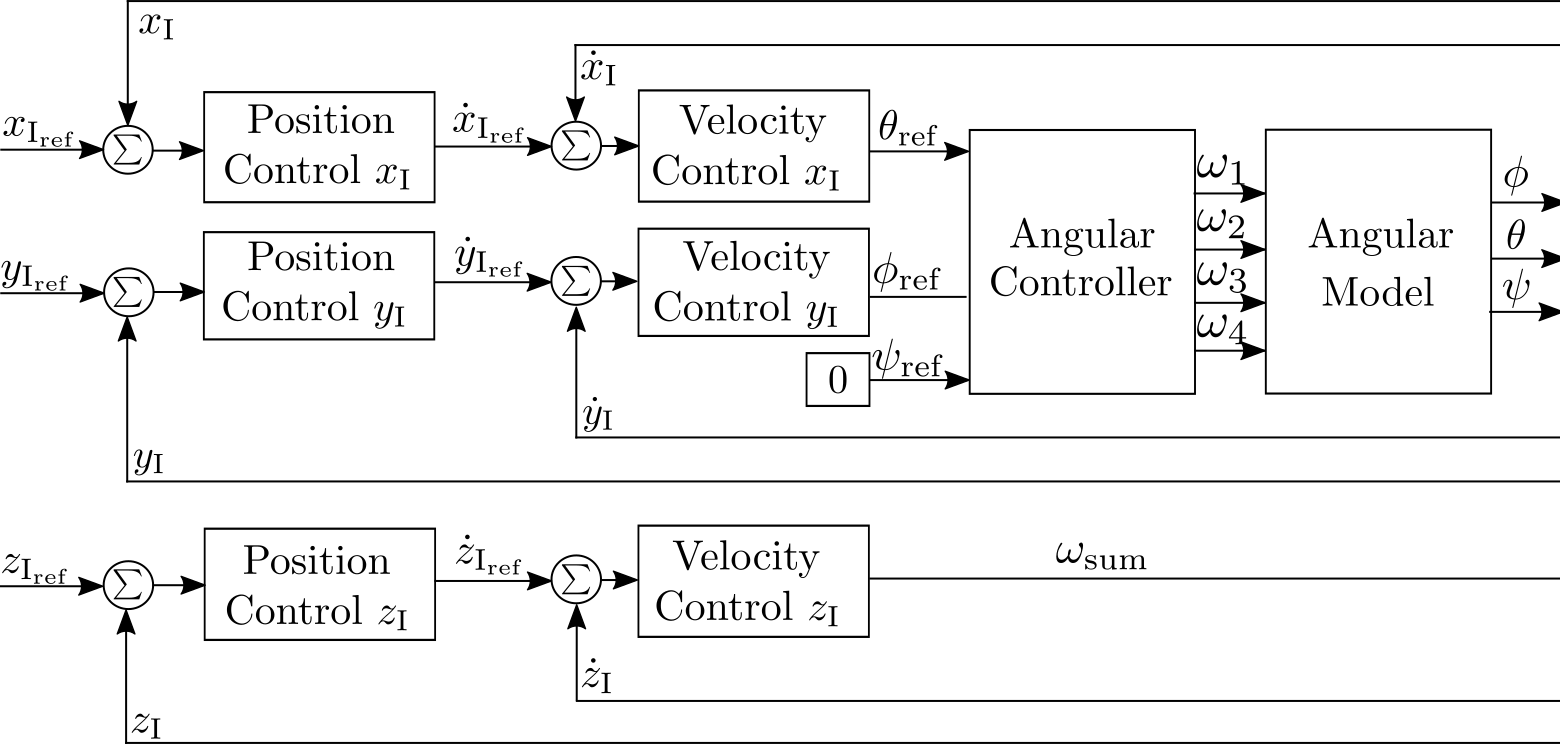
\includegraphics[width=0.88\linewidth]{figures/TranslationalControlDiagram}
	\caption{Diagram of the control solution.}
\end{figure}

\begin{columns}[t,totalwidth=\twocolwid] % Split up the two columns wide column

	\begin{column}{0.43\twocolwid} % The first column within column 2 (column 2.1)
  	 \centering
  	 \hspace{-2cm}
  	 \parbox{.88\textwidth}{
    	 \begin{itemize}
  	 			\item[]\textbf{Attitude controller}\\
  	 			\item State feedback with integral control using LQR is designed for tracking references and handling disturbances.
  	 			\item A reduced order observer is used to estimate the angular velocities.
  	 		\end{itemize}
  	 }
	\end{column} % End of column 2.1
	\hspace{-4cm}
	\begin{column}{0.57\twocolwid} % The second column within column 2 (column 2.2)
  	 \centering
   	 \parbox{1\textwidth}{
       	 \begin{itemize}
    	 			\item[]\textbf{Translational controllers}\\
     	 			\item PI controllers are used to control the velocities in order to handle input disturbances.
     	 			\item The outer loops are P controllers used to control the positions.
     	 			\item The bandwidths of the cascaded controllers are considered to reduce the effect of the dynamics of the inner loops in the outer loops.
       	 \end{itemize}		
   	 }
	\end{column} % End of column 2.2
	\vspace{-.5cm}
\end{columns} % End of the split of column 2 - any content after this will now take up 2 columns width